\documentclass[10pt]{beamer}

\usepackage{amsfonts}
\usepackage{subfiles}
\usepackage[T2A]{fontenc}
\usepackage[utf8]{inputenc}
\usepackage[russian]{babel}

\usepackage{amsmath, amsfonts, amssymb, amsthm, mathtools, mathrsfs}
\usepackage{wasysym, dsfont}
\usepackage{graphicx}
\usepackage{float}
\usepackage{wrapfig}

\usepackage{caption}
\usepackage{subcaption}
\usepackage{longtable}
% \usepackage{subfigure}

\usepackage{multicol}
\DeclareMathOperator*{\argmax}{\arg\!\max}
\DeclareMathOperator*{\argmin}{\arg\!\min}

\mode<presentation>
{
	\usetheme{boxes}
	\beamertemplatenavigationsymbolsempty
	
	\setbeamertemplate{footline}[page number]
	\setbeamersize{text margin left=1.5em, text margin right=2.0em}
}
\newcommand\blfootnote[1]{%
	\begingroup
	\renewcommand\thefootnote{}\footnote{#1}%
	\addtocounter{footnote}{-1}%
	\endgroup
}
\newcommand\FontUP{\fontsize{12}{12}\selectfont}


\title[]{Обучение взаимосвязанных информативных представлений в задаче генерации образов}
\author{Охотников Никита Владимирович}
\institute{МФТИ}
\date{2023-2024}


\begin{document}

\begin{frame}
  \titlepage
\end{frame}


\begin{frame}
	\frametitle{Введение}
	Исследуется задача поиска наилучшего дополнения образа --- множества взаимосвязанных элементов (на примере элементов одежды) --- элементами конечной коллекции.
	\begin{block}{Проблемы}
		\begin{itemize}
			\item Взаимосвязь элементов в образе имеет неизвестную структуру.
			\item Точное решение задачи дополнения требует полного перебора.
		\end{itemize}
	\end{block}
	\vfill
	\begin{block}{Задача}
			Предложить применимый на практике приближенный алгоритм дополнения образа несколькими элементами.
	\end{block}	

	\vfill
	\begin{block}{Предлагается}
		На основе известной функции оценки образа построить функцию для генерации зависимых скрытых представлений элементов, использующихся далее для выбора элементов дополнения на основе близости в латентном пространстве.
	\end{block}	
\end{frame}


\begin{frame}
	\frametitle{Постановка задачи}
		\begin{block}{Основные понятия и обозначения}
			\begin{itemize}
				\item Основная единица данных, рассматривающаяся в работе -- элемент одежды, далее будем называть его \textit{объектом} или \textit{элементом}, множество всех рассматриваемых объектов -- $\mathcal{X}$
				
				\item Каждый объект $X\in\mathcal{X}$ есть пара $X = (I, T)$ из соответственно изображения о текстового описания.  
				\item Далее под объектом $X\in \mathcal{X}$ будем понимать его векторное представление $X\in\mathbb{R}^d$ в общем для всех элементов признаковом пространстве.								
				\item Непустые подмножества множества элементов $O = \{X_i\}_{i=1}^k\subset \mathcal{X}, O\neq\{\O\}$ будем называть \textit{образами}. Множество образов обозначим $\mathcal{O}$.
				\item Для оценки образов введем функцию \textit{оценки} или \textit{совместимости} его элементов: 
				$$\mathcal{S}:~2^\mathcal{X}\longrightarrow [0,1]$$
				$$\forall O \in \mathcal{O}:~\mathcal{S}(O) > 0$$
				\textit{Совместимостью} или \textit{оценкой} образа $O$ будем называть $\mathcal{S}(O)$
			\end{itemize}
		\end{block}					
\end{frame}

\begin{frame}
	\frametitle{Постановка задачи}
	\begin{block}{Задача дополнения образа}
		\begin{itemize}
			\item \textbf{Дано:}\\
			$O_n\in\mathcal{O}, ~|O| = n$ --- исходный образ \\
			$k \in \mathbb{N}, ~k$ --- количество элементов дополнения \\	
			
			\item \textbf{Требуется:}\\
			Найти наилучшее в смысле максимизации функции оценки $\mathcal{S}$ дополнение образа $O_n$  $k$ элементами $\{\hat{X_i}\}_{i=1}^k\subset \mathcal{X}$ т.е. решить следующую оптимизационную задачу
			$$\{\hat{X_i}\}_{i=1}^k= \argmax_{\{X_i\}_{i=1}^k\subset\mathcal{X}} \mathcal{S}\left(O_n\cup\{X_i\}_{i=1}^k\right)$$
			\item  Точное решение для известной $\mathcal{S}$: полный перебор всех подмножеств $\mathcal{X}$ размера $k$.\\
			Асимптотика: $|\mathcal{X}|^k$ вызовов функции $\mathcal{S}$
		\end{itemize}
	\end{block}					
\end{frame}


%\begin{frame}
%	\frametitle{Постановка задачи}
%	\begin{block}{Оценка образа}
%		Задача оценки образа -- это классическая задача регрессии направленная на получения аппроксимации функции оценки $ \mathcal{S}$: \\
%		\begin{itemize}
%			\item \textbf{Дано:}\\
%			$\{O_1\dots O_n\}\subset \mathcal{O}$\\
%			$\{\mathcal{S}(O_1)\dots\mathcal{S}(O_n)\}$
%			\item \textbf{Требуется:}\\
%			Найти наилучшую в некотором смысле аппроксимацию функции $\mathcal{S}$ функциями заданного класса, т.е. решить задачу оптимизации:\\
%			$$\hat{\mathcal{S}}= \argmin_{S\in\mathscr{S}}\left[\frac{1}{N} \sum\limits_{i=1}^N\mathcal{L}(\mathcal{S}(O_i), S(O_i))\right]$$
%			где $\mathcal{L}(\cdot, \cdot)$ некоторая метрика, например евклидова, а $\mathscr{S}$ -- рассматриваемое множество функций, например нейросети заданной архитектуры.
%		\end{itemize}
%	\end{block}					
%\end{frame}
%
%
%\begin{frame}
%	\frametitle{Постановка задачи}
%	\begin{block}{Описание образа}
%		Задача описания образа есть задача построения наилучшего текстового описания для данного образа по изображениям его элементов. Полагая функцию оценки известной получаем:\\
%		\begin{itemize}
%			\item \textbf{Дано:}\\
%			$\{X_i\} = O_n, ~|O_n| = n$ --- образ, где $X_i = (I_i, \O),~I_i\in\mathcal{I},~i=\overline{1, n}$ --- его элементы с пустым текстовым описанием. \\
%			$O_n(T) = \{X_i(T) = (I_i, T)\}_{i=1}^n$ для некоторого общего описания $T$\\
%			\item \textbf{Требуется:}\\
%			Найти оценку $\hat{T}$ общего для всех элементов описания $T$, максимизирующую значение функции оценки $\mathcal{S}(O_n)$, т.е.: \\
%			$$\hat{T}= \argmax_{T}\mathcal{S}(O_n(T))$$
%		\end{itemize}
%		В данном случае задача генеративная --- лучшее описание находится, из решения задачи максимизации функции оценки, а не просто выбирается из заранее заданного конечного множества.
%	\end{block}					
%\end{frame}
%
%
%\begin{frame}
%	\frametitle{Постановка задачи}
%	\begin{block}{Дополнение (восстановление) образа}
%		Задача дополнения образа -- есть задача выбора в некотором смысле наилучшего набора элементов из $\mathcal{X}$ для дополнения данного образа:
%		\begin{itemize}
%			\item \textbf{Дано:}\\
%			$O_n\in\mathcal{O}, ~|O| = n$ \\
%			$k \in \mathbb{N}, ~k> n$ --- количество недостающих элементов\\
%			$J\subset\mathbb{N},~|J| = m\geqslant k$ --- индексы категорий недостающих элементов\\
%			$\{\hat{T_i}\}_{i=1}^k$ --- текстовые представления недостающих элементов, возможно пустые. В случае если предлагается только текстовое описание всего образа $T$, рассматривается $\forall i \in \overline{1,k}: ~T_i = T$.
%			
%			\item \textbf{Требуется:}\\
%			Найти наилучшее в смысле максимизации функции оценки дополнение образа $O_n$ до $O_k\in\mathcal{O}, |O_k|=k$ элементами из категорий $\{C_j\}_{j\in J}$, т.е. решить следующую задачу:
%		\end{itemize}
%	\end{block}					
%\end{frame}
%
%
%\begin{frame}
%	\frametitle{Постановка задачи}
%	\begin{block}{Дополнение (восстановление) образа}
%		$$\{\hat{X_i}\}_{i=1}^k= \argmax_{\{X_i\}_{i=1}^k\in\bigcup\limits_{j\in J}\mathcal{X}_{C_j}} \bigg{[}\alpha \cdot \mathcal{S}\left(O_n\cup\{X_i\}_{i=1}^k\right) + $$
%		
%		$$+ (1-\alpha) \cdot \sum\limits_{i=1}^k S_X((I_i, T_i), (I_i, \hat{T_i}))\cdot\mathbb{I}\{\hat{T_i}\neq\O\}  \bigg{]}$$				
%		здесь $X_i = (I_i, T_i)$, $\alpha\in[0,1]$. Второе слагаемое отвечает за соответствие предсказанного элемента предъявленному текстовому представлению и равно нулю, если представление пусто. Задача, в отличие от предыдущей, дискриминативная и  может быть решена точно полным перебором всех объектов из $\mathcal{X}$.
%	\end{block}					
%\end{frame}
%
%
%\begin{frame}
%	\frametitle{Постановка задачи}
%	Задача генерации состоит в выборе образа произвольного размера, наиболее подходящего к предоставленному текстовому описанию. В терминах введенных выше получаем:
%	
%	\begin{itemize}
%		\item \textbf{Дано:}\\
%		$T$ --- текстовое описание образа.
%		
%		\item \textbf{Требуется:}\\
%		Найти наилучший в смысле максимизации функции оценки образ $O\in\mathcal{O}$ элементы которого наилучшим образом соответствуют предложенному описанию $T$, т.е.:
%		$$ \hat{O} = \argmax_{k,O = \{X_i\}_{i=1}^{k},  O\in\mathcal{O}} \left[\alpha \cdot \mathcal{S}(O) + (1-\alpha) \cdot \sum\limits_{i=1}^{k} S_X((I_i, T_i), (I_i, T))\cdot\mathbb{I}\{\hat{T}\neq\O\}  \right]$$				
%		здесь $X_i = (I_i, T_i)$, $\alpha\in[0,1]$. 
%		Стоит заметить, что если зафиксировать $k=1$, получаем обычную задачу поиска наиболее подходящего под описание элемента в коллекции. Учитывая то, что множество образов определено множеством элементов и определением образа, задача генерации образа также является дискриминативной и состоит в переборе всех возможных образов.
%	\end{itemize}			
%\end{frame}


\begin{frame}
	\frametitle{Теоретическая часть}
	\begin{itemize}	
	 	\item В качестве аппроксимации функции оценки $\mathcal{S}$ далее будем рассматривать предобученную модель OutfitTransformer\footnote{\url{https://doi.org/10.48550/arXiv.2204.04812}}.
	    \item Для задачи дополнения 
	    $$\{\hat{X_i}\}_{i=1}^k= \argmax_{\{X_i\}_{i=1}^k\subset\mathcal{X}} \mathcal{S}\left(O_n\cup\{X_i\}_{i=1}^k\right)$$
	    существует 2 глобальных подхода 
	    \begin{itemize}	
	    	\item Дискретный -- оптимизация полного перебора
	    	\item Непрерывный -- решение релаксированной задачи в $\mathbb{R}^d$ и поиск ближайших к решению элементов $\mathcal{X}$
	    \end{itemize}
	   \end{itemize}
\end{frame}


\begin{frame}
	\frametitle{Дополнение образа}
	\begin{block}{Дискретный подход}
		\begin{itemize}
			\item Решение задачи приближенным перебором
%			\item Рассмотрим полный граф на вершинах $\mathcal{X}\setminus O_n \cup \{X_{init}\}$, где $X_{init}$ -- дополнительная начальная вершина. \\
%			Тогда задача дополнения эквивалентна максимизации \textit{оценки} пути $X_{init}, X_1, X_2\dots X_k$ в таком графе. Где \textit{оценкой} пути --- оценка образа $O_n\cup\{X_1\dots X_k\}$
			\item Бейзлайн: жадные алгоритмы
			\begin{itemize}
				\item[<<1-step>>] $X_1 = \argmax\limits_{X\in\mathcal{X}}{\mathcal{S}(O_n\cup X)},~\dots , X_k = \argmax\limits_{X\in\mathcal{X}\setminus \bigcup\limits_{i=1}^{k-1} X_i} \mathcal{S}(O_n\cup X)$\\
				Асимптотика: $|\mathcal{X}|$ вызовов функции $\mathcal{S}$\\
				
				\item[<<k-step>>] $X_1 = \argmax\limits_{X\in\mathcal{X}}{\mathcal{S}(O_n\cup X)},~\dots , X_k = \argmax\limits_{X\in\mathcal{X}\setminus \bigcup\limits_{i=1}^{k-1} X_i} \mathcal{S}(O_n\cup X_1\dots X_{k-1}\cup X)$\\
				Асимптотика: $k\cdot|\mathcal{X}|$ вызовов функции $\mathcal{S}$
			\end{itemize}
				
			\item Альтернатива: алгоритм beam-search, активно применяемый в языковых моделях. В граничных случаях вырождается либо в полный перебор, либо в k-step алгоритм выше.\\
			Асимптотика:  $\geqslant k\cdot|\mathcal{X}|$ вызовов функции $\mathcal{S}$
		\end{itemize}
	\end{block}
\end{frame}


\begin{frame}
	\frametitle{Дополнение образа}
	\begin{block}{Непрерывный подход (градиентный спуск)}
		\begin{itemize}
			\item Функция $\mathcal{S}$ непрерывно дифференцируема почти всюду и с ограниченным по норме градиентом, а значит липшицева с некоторой константой $M$
			\item Есть доступ не только к значению функции оценки, но и к ее градиенту 
			\item Идея: заменим дискретную задачу непрерывной:
			 	$$\{\tilde{X_i}\}_{i=1}^k= \argmax_{\{X_i\}_{i=1}^k\subset\mathbb{R}^d} \mathcal{S}\left(O_n\cup\{X_i\}_{i=1}^k\right)$$
	 \item Далее выберем $\{\hat{X_i}\}\subset\mathcal{X}$ как ближайшие к решениям  в смысле функции близости $\rho$:
	 \vspace{-0.3cm}
	 $$\hat{X_i} =  \argmin_{X\in\mathcal{X}} \rho(\tilde{X_i}, X)$$
	  \vspace{-0.5cm}
	 \item Полученная задача разрешима за разумное время с помощью стохастического градиентного спуска.
	 \item Асимптотика $n$ вызовов функции оценки и ее градиента, где $n$ -- количество шагов градиентного спуска (не зависит от $|\mathcal{X}|$)
		\end{itemize}
	\end{block}
\end{frame}


\begin{frame}
	\frametitle{Дополнение образа}
	\begin{block}{Непрерывный подход (градиентный спуск)}
		\begin{itemize}
			\item $\mathcal{S}$ -- $M$-липшицева
			\item рассмотрим $L_p$ метрику в качестве $\rho$, тогда
			$$\sum_{i=1}^k\rho(\hat{X_i}, \tilde{X_i}) < \varepsilon\longrightarrow \biggr{|}\mathcal{S}\left(O_n\cup\{\tilde{X_i}\}_{i=1}^k\right) - \mathcal{S}\left(O_n\cup\{\hat{X_i}\}_{i=1}^k\right)\biggr{|} < M\cdot\varepsilon$$
			
			\item Проблема подхода: $\exists\{\hat{X_i}\}\subset \mathcal{X}:~ \sum\limits_{i=1}^k\rho(\hat{X_i}, \tilde{X_i}) < \varepsilon$ --- очень сильное условие и требует по крайней мере
			$$\exists \{\hat{X_i}\}_{i=1}^k\subset\mathcal{X}:~ \mathcal{S}\left(O_n\cup\{\hat{X_i}\}_{i=1}^k\right) \geqslant \max_{\{X_i\}_{i=1}^k\subset\mathbb{R}^d} \mathcal{S}\left(O_n\cup\{X_i\}_{i=1}^k\right) - M\varepsilon$$
			$$\Updownarrow$$
			$$\max_{\{X_i\}_{i=1}^k\subset\mathcal{X}} \mathcal{S}\left(O_n\cup\{X_i\}_{i=1}^k\right) \geqslant \max_{\{X_i\}_{i=1}^k\subset\mathbb{R}^d} \mathcal{S}\left(O_n\cup\{X_i\}_{i=1}^k\right) - M\varepsilon$$
		\end{itemize}
	\end{block}
\end{frame}

\begin{frame}
	\frametitle{Дополнение образа}
	\begin{block}{Непрерывный подход (генерация скрытых представлений)}
		\begin{itemize}
			\item Предлагается \textit{полностью} отказаться от вызовов функции $\mathcal{S}$
			\item Переформулируем задачу как поиск аппроксимации функции 
			$$\mathcal{F}_k: \mathcal{O}\longrightarrow \mathcal{X}^k, ~~~O_n\in \mathcal{O},~ \mathcal{F}_k(O_n) = \argmax_{\{X_i\}_{i=1}^k\subset\mathcal{X}} \mathcal{S}\left(O_n\cup\{X_i\}_{i=1}^k\right)$$
			Композицией функций 
			$$F_k^\theta: \mathcal{O}\longrightarrow \mathbb{R}^d, ~F_k^\theta(O_n) = \{\tilde{X_i}\}_{i=1}^k$$
			$$\text{и }\rho_\mathcal{X}: \mathbb{R}^d\longrightarrow \mathcal{X}, ~ \rho_\mathcal{X}(\tilde{X_i}) = \argmax_{\hat{X_i}\in\mathcal{X}}\rho(\tilde{X_i}, \hat{X_i})$$
			\item $d \gg 1$ поэтому далее, следуя рекомендациям из статьи\footnote{\url{https://journals.plos.org/plosone/article?id=10.1371/journal.pone.0144059}} будем в эксперименте использовать в качестве $\rho$ косинусную близость
		\end{itemize}
	\end{block}
\end{frame}


\begin{frame}
	\frametitle{Дополнение образа}
	\begin{block}{Непрерывный подход (генерация скрытых представлений)}
		\begin{itemize}
			\item Свели исходную задачу к задаче генерации скрытых представлений недостающих элементов $\{\tilde{X_i}\}\subset \mathbb{R}^d$, наиболее близких в смысле функции $\rho$ к точным решениям задачи
			$$\{\hat{X_i}\}_{i=1}^k= \argmax_{\{X_i\}_{i=1}^k\subset\mathcal{X}} \mathcal{S}\left(O_n\cup\{X_i\}_{i=1}^k\right)$$
			с помощью функции  $F_k^\theta$ с вектором параметров $\theta$. 
			\item Рассмотрим образы $\mathcal{O}_n = \{O^i\}_{i=1}^n \subset\mathcal{O}$ и множество известных точных решений задачи дополнения для них $\mathcal{X}_n =\{\{\hat{X_j^i}\}_{j=1}^k\}_{i=1}^n\subset\mathcal{X}^k$
			\item Тогда на параметры $\theta$ получаем следующую оптимизационную задачу:
			$$\theta = \argmin_{\hat{\theta}}\left( \frac{1}{n}\sum_{i=1}^n\sum_{j=1}^k\rho\left(X_j^i, [F_k^{\hat{\theta}}(O^i)]_j\right)\right)$$
		\end{itemize}
\end{block}
\end{frame}


\begin{frame}
	\frametitle{Дополнение образа}
	\begin{block}{Непрерывный подход (генерация скрытых представлений)}
		\begin{itemize}
			\item  Задача симметрична к перестановке $\Longrightarrow$ разумно рассматривать операции эквивариантные относительно группы перестановок.
			\item Тогда представим функцию $F_k^\theta$ с помощью графовой нейронной сети (GNN)
			\item Вершины графа --- представления элементов образа
			\item Общий вид преобразования $h_i^{(t)}$ скрытого состояния $i$-ой вершины на шаге $t$ в message passing GNN\footnote{https://arxiv.org/pdf/1704.01212}:
			$$h_i^{(t)} = \gamma^{(t)} \left(h_i^{(t-1)}, \bigoplus\limits_{j\in \overline{1, n}}\phi^{(t)} \left(h_i^{(t-1)}, h_j^{(t-1)} \right) \right),$$
			где $\gamma^{(t)}, \phi^{(t)}$ -- дифференцируемые функции, $\bigoplus$ --- дифференцируемая аггрегирующая функция, инвариантная к перестановкам (в эксперименте будем использовать сумму)
		\end{itemize}
	\end{block}
\end{frame}

\begin{frame}
	\frametitle{Дополнение образа}
	\begin{block}{Непрерывный подход (генерация скрытых представлений)}
		\begin{itemize}
			\item Асимптотика: один вызов функции $F_k^\theta$
			\item Аппроксимация напрямую решений дискретной, а не релаксированной задачи
			\item Позволяет получать произвольное количество скрытых представлений для элементов дополнения за один проход
			\item Моделирует зависимости между элементами дополнения
			\item В качестве $\mathcal{X}_n$ можно рассмотреть набор решений задачи многошаговым жадным алгоритмом
		\end{itemize}
	\end{block}
\end{frame}


\begin{frame}
	\frametitle{Вычислительный эксперимент}
	\begin{block}{Условия эксперимента}
		\begin{itemize}
			\item Данные: датасет Polyvore\footnote{http://arxiv.org/abs/1707.05691} --- 17000 образов из 65000 объектов
			\item Случайно выберем 1000 образов 
			\item Зафиксируем количество элементов дополнения $k=2$
			\item Оцениваем алгоритмы на основании распределения оценок дополненных образов
			\item Бейзлайн: рапределение оценок исходных образов
		\end{itemize}
	\end{block}
\end{frame}


\begin{frame}
	\frametitle{Вычислительный эксперимент}
	\begin{block}{Дискретный подход (жадные алгоритмы)}
		\vspace{0.3cm}
		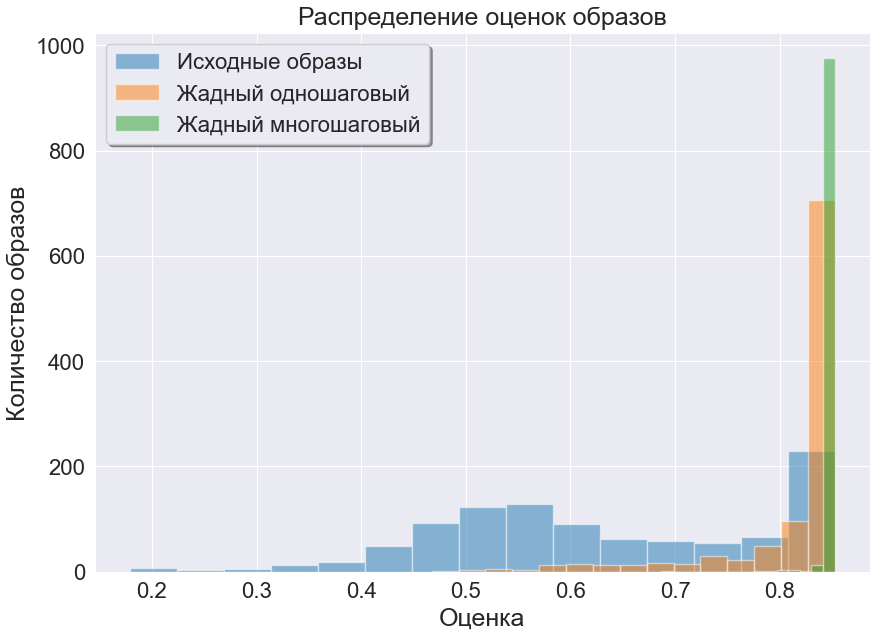
\includegraphics[scale = 0.5]{../figures/greedy_at_least_5_subset1000.png}
		
		Показывают хороший результат, но требуют слишком много времени
	\end{block}
\end{frame}

\begin{frame}
	\frametitle{Вычислительный эксперимент}
	\begin{block}{Непрерывный подход (градиентный спуск)}
		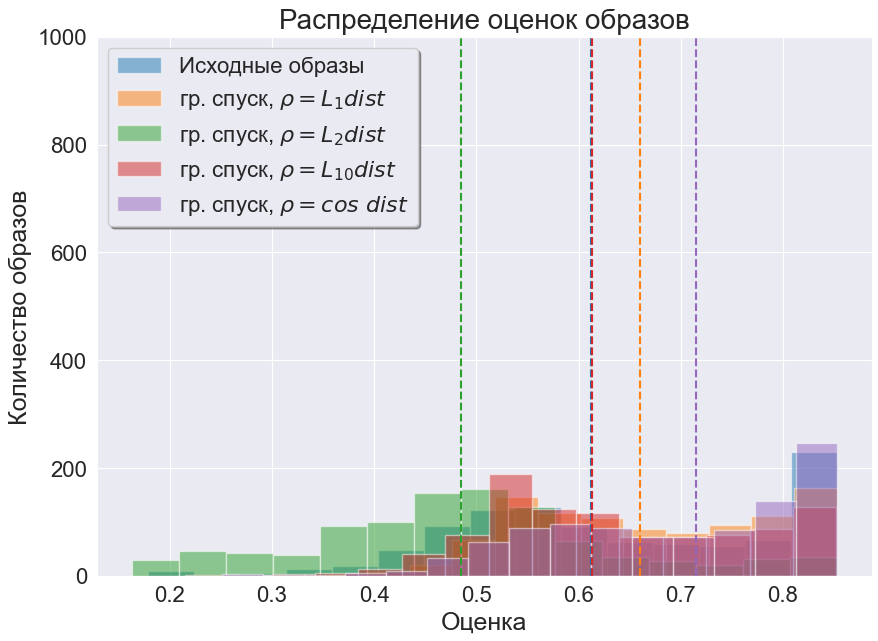
\includegraphics[scale = 0.5]{../figures/backprop_at_least_5_subset1000.png}
	\end{block}
Результат заметно хуже чем для жадных алгоритмов, а время вычислений все еще не позволяет использовать такой подход на практике
\end{frame}

\begin{frame}
	\frametitle{Вычислительный эксперимент}
	\begin{block}{Непрерывный подход (генераций представлений)}
		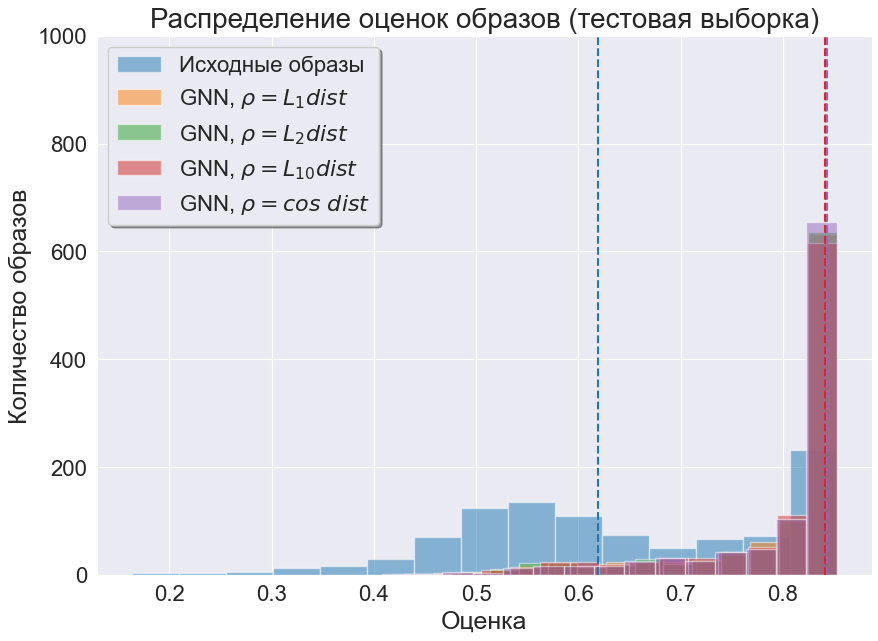
\includegraphics[scale = 0.5]{../figures/GNN_at_least_5_subset1000_test.png}
	\end{block}
\end{frame}


\begin{frame}
	\frametitle{Выносится на защиту}
		\begin{itemize}
			\item Предложен эффективный алгоритм дополнения образа произвольным числом взаимосвязанных элементов
			\item Предложен способ пополнения обучающих данных для модели в условиях недостатка образов с высокой оценкой
			\item Реализован программный код для вычислительного эксперимента и проведена оценка предложенных подходов				
		\end{itemize}
\end{frame}




\end{document}
